%WISDOM TO ALL:
%FUCK THIS SHIT; REPORTS ARE SHIT, NOT THE SHIT

%\documentclass[norsk,a4paper,12pt]{article}

\documentclass[%
 reprint,
 amsmath,amssymb,
 aps,
 norsk
]{revtex4-1}

\usepackage{graphicx}% Include figure files
\usepackage{dcolumn}% Align table columns on decimal point
\usepackage{bm}

\usepackage[T1]{fontenc} %for å bruke æøå
\usepackage[utf8]{inputenc}
\usepackage{graphicx} %for å inkludere grafikk
\usepackage{verbatim} %for å inkludere filer med tegn LaTeX ikke liker
\usepackage{mathpazo}
\bibliographystyle{plain}

%\usepackage{lstlistings}

%\usepackage{subfig}
%\usepackage{caption}

\usepackage{graphicx} %subigure
\usepackage{subcaption}


\usepackage{color}
\definecolor{pink}{RGB}{219, 48, 122}

%\usepackage{siunitx} %\ang{num}
\usepackage{textcomp}

\usepackage{geometry}
 \geometry{
 a4paper,
 total={170mm,257mm},
 left= 30mm,
 right = 30mm,
 bottom = 30mm,
 top=30mm	}
 

%\preprint{APS/123-QED}
%\title{Manuscript Title}% Force line breaks with \\
%\thanks{A footnote to the article title}%

%\author{Ann Author}
% \altaffiliation[Also at ]{Physics Department, XYZ University.}
% \email{Second.Author@institution.edu}

%\collaboration{CLEO Collaboration}%\noaffiliation

             
\begin{document}  
        
\title{Summer school - needs proper title}
\author{Marianne Bjerke, University of Oslo}
\date{\today}
%\date{April 2018}%\today}



\begin{abstract}

Oslo method, MAMA, REINIER

%\begin{description}
%\item[Usage]
%Secondary publications and information retrieval purposes.
%\item[PACS numbers]
%May be entered using the \verb+\pacs{#1}+ command.
%\item[Structure]
%You may use the \texttt{description} environment to structure your abstract;
%use the optional argument of the \verb+\item+ command to give the category of each item. 
%\end{description}

\end{abstract}

\maketitle
\tableofcontents


%\tableofcontents

\section{Theory}

\subsection{Nuclear level density}

This is a measurement on how many states there are per MeV. Higher levels also have a width $\Gamma$. If the level spacing is $D$ then the level densities can be discrete ($\Gamma << D $), a quasi continuum ($\Gamma \leq \ D $) or a continuum ($\Gamma \geq \ D $). In the hight energies you will also get mixing and ressonances of the states. The discrete levels are  fairly easy to measure (eg. by measuring distinct gamma energies from decay), but in the semi- and continuum the energy levels are so close it is essentially impossible to actually find specific ones. 

\begin{equation}
\Delta E \Delta t \leq \frac{\hbar}{2} \Rightarrow \Gamma \propto \frac{1}{\tau}
\end{equation}

% ILLUSTRATION.

\subsection{Spin distribution}



\subsection{Brink-Axel hyothesis and Porter-Thomas fluctuations}
The Brink-Axel (gBA) hypothesis states that the absorption and emission in decay and exitation of nuclei are only dependent on $E_{\gamma}$ and is independent on the initial and final $E_x$ as well as the spin/parity of these states. 

Often assumed when calculating gamma ray strength functions. Folksy: The nucleus "looks" exactly the same for a photon being absorbed on the ground state or any other excuted state.


Porter-Thomas fluctuations. The distribution in the liit f extreme configuration mixing. (chi squared(?)) 

A solution might be that a generalized Brink-Axel may be the underlying principle, but that it's camouflaged by Porter-Thomas fluctuations due to fe transitions.

gBA is better for heavy systems. For lighter systems, the individual gamma str. func. are centered around a common gamma s.f. The deviations are driven by som e sort of fluctuations.



\subsection{Reduced transition probability}
\subsection{$\gamma$-ray strength function}

Ann-Cecilie: What IS the gamma-ray strengsth function? A measure of the average, reduced gamma decay probability. Below particle thresholds (the energy needed to rip out a neutron or proton) the nucleus decays via gamma emission, and the probability of gamma decay tels us a lot about the structure and dynamics of the nucleus.

Why is it important and what can we learn from it? Deviations from single-particle (constant) ecay strength. Resonant behaviour of gamma-absorption and decay(Giant Dipole Resonance, M1 scissors  mode, M1 spin-flip resonance.)

Does a common $\gamma$-ray strength function even exist? That is the question. A unique and smooth gammastrenght function would simplify calculations a lot. The gamma strength from some transitions are a bit "unpredictible".


\begin{figure}
	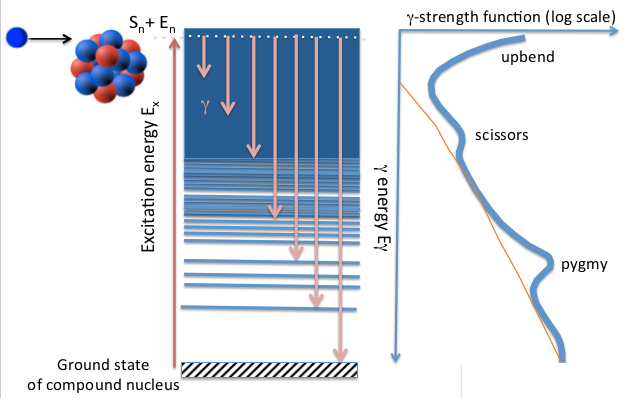
\includegraphics[angle=0, width = 75mm]{gammastr_anncecilie.png}
	\caption{ Gamma strength function. From Ann-Cecilies lecture and presentation on the gamma strength function. \label{fig:gammastr_anncecilie}}
\end{figure}

The gamma str. func. can have a few features. They always have a Giant electric dipole (GDR) resonance which is split if the nucleus is deformed. It can possibly have a giant magnetic dipole resonance (GMDR), an electric pygmy dipole resonance (PDR), possible M1 scissors resonance (in deformed nuclei) and low-energy enchantment, upbend, low-energy increase etc.









\subsection{Iterative unfolding}
The need for unfolding data arises from the fact that the signal from the detector is composed of more than the signal we are looking for itself. 
This includes a Compton scattering peak, full energy peak, single escape peak, double escape peak, $511$ keV peak, backcatter peak and electrical background noise in the sensors and electronics.

To unfold sucsessfully you need a response matrix for the detector. It it quite common to find interaction probabilities by Mone-Carlo simulations of the specific detector system. This response matrix works so that the true spectrum of $\gamma$-rays $\mathbf{x}$ and detector signal $\mathbf{y}$ is correlated by $\mathbf{y} = \mathbf{Ax}$.



\subsection{Cooper pairs}

what are they?? Spin paired nucleons?

Cooper pais usually describes electrons and it's the description of a quantum pairing. 

Paired nucleons as well?







\subsection{First generation gammas of the oslo method.}
According to M Guttormsen et al. \cite{guttormsen_firstgenerationgamma} the present method is based on the assuption that states populated after the first $\gamma$-transition have the same decay propertie as states populated directly in the partivle reaction at that excitation energy. The assumption seems to be fulfilled inthe regions ofhigh density. The $\gamma$decay also seems to consist of sstatistical dipole radiationcarrying a vanishing spin transfer on average in the continuum.

For each excitation region (bin) rpoduced form the partivle-$\gamma$ coincidences a gamma-ray spectrum denoted $f_i$. The first gen.  gammaray spectrum f the highest excitation energy (bin no. 1) is estimated by $h = f_1 - g$ where g is a weighted sum of all spectra
\begin{equation}
g = \Sigma_i n_i w_i f_i
\end{equation}

Coeff. $w_i$ are unknownand represent the probability $\Sigma w_i = 1$ of the decay from bin 1 to bin i.



AFTER GETTING SOME KNoWLEDGE! 
First generation $\gamma$-spectra are the first decays after an exitation. What is ideally done is to excite all nuclei to the same (high) exitation level and record the $\gamma$-decays to extract only the first $\gamma$ decays directly from that beginning state. See the middle illustration of fig. \ref{fig:gammastr_anncecilie}. The problem is separating the first generation spectra from the subsequent ones, as only some might decay straight to the ground state, which will have some of the same energies as the first generation ones.

The first-generation method works iterative by summing over weighted spectra\cite{guttormsen_firstgenerationgamma}. COPY STUFF FROM ABOVE.

\subsection{Motivation}
When it might be interesting and most useful to describe the behaviour of atomic nclei with average properties rather than properties of discrete levels.


\section{Shell model calculations}







\subsection{Calculating gamma ray strength functions and nuclear level density using shell model.}





\section{Software}

\subsection{A note on previously exiting softare}
TALYS, for exmple, has previously been used 
.. and as stated in the abstract of \cite{Kirsch_RAINIER}.
"modern reaction codes such as TALYS and EMPIRE populate a wide range of states in the residual nucleus prior to $\gamma$-sray decay, but do not go beyond the use of deterministic functions and therefore neglect cascade fluctuations."

This show us an underlying problem with some examples of previously used software as cascades of nuclear reactions might be statistially predictable though highly undeterministic. 


\subsection{RAINIER}

(13.) What it is and what it can do.

RAINIER calculates random, discrete, gamma emission in the semi-continuum of the nuclear level density. It is also randomised and Monte-Carlo based (??). 

It is only intended for $\gamma$ rays and is therefore only in bound states/energy levels (exitation is low enough so the nucleus only emmit gammas and not $\alpha$'s or other particles. 

This wil produce synthetic data we can analyze with the MAMA software (Oslo method).


The low energy portions of the level scheme (the discrete and well known states) is supplied from other sources (eg. TALYS?). We then populate higher level(s?) and look at the cascade it produces. 

\subsection{Oslo method}



\subsection{the beta-Oslo method}

Continued:

Carl Sagans starstuff-quote.

















\begin{figure}
	%\includegraphics[angle=0, width = 75mm]{plot_trefilter.png}
	\caption{Plot av $\theta$ for filter 2 vs. intensitet for oppsett med tre polarisasjonsfiltre. Filter 1 og 3 er satt på $0$\textdegree og $90$\textdegree respektivt. Se oppsett i fig \ref{fig:trefilter_skisse} \label{fig:plot_trefilter}}
\end{figure}


\begin{table}
	\centering
	\begin{tabular}{ c c } 		
	Grader & E[lux] \\
	$0$\textdegree  & $156$ \\
	$10$\textdegree & $153$ \\
	$20$\textdegree & $141$ \\
	\end{tabular}
	\caption{caption \label{tab:II_twofilters}}
\end{table}




%\end{multicols}

\begin{thebibliography}{9}
%\bibitem{Squires}
%G.L. Squires - Practical Physics, fourth edition (Cambridge, 2001)
%\bibitem{lokalg} 
%Montana State University, \\
%\textit{physics.montana.edu/demonstrations/video/1\_mechanics/demos/localgravitychart.html},
%hentet 6. februar 2018. 

\bibitem{Calcite_birefringence}
Eksempel på dobbeltbrytning i kalsittkrystall. Hentet 1.juni 2018 fra http://www.quirkyscience.com/wp-content/uploads/2015/09/Calcite-Splitting.jpg

%HOW THE F DO YOU DO THIS PROPERLY?
\bibitem{Kirsch_RAINIER} Paper: RAINIER: A simulation tool for distributions of excited nuclear states and cascade fluctuations
L.E. Kirsch, L.A. Bernstein

\bibitem{guttormsen_firstgenerationgamma} Paper: The first generation of gamma-rays formhot nuclei.

\bibitem{test} test here

\end{thebibliography}





%\bibliography{referanser}
\end{document}
